\section{Auswertung}
\label{sec:auswertung}

Es folgt die Auswertung der unterschiedlichen
Versuchsteile mit allen relevanten Messdaten.

Die Unsicherheit für abgeleitete Größen wurden mit der Fehlerfortpflanzung \eqref{eq:gaussf} berechnet bzw. mit dem "uncertainties" package der Programmiersparche Python.

\begin{equation}
Δf(x_1,...,x_N)=\sqrt{\sum_{i=1}^N (\frac{\partial f}{\partial x_i}Δx_i)^2}
\label{eq:gaussF}
\end{equation}


\subsection{Charakteristik des Zählrohres}
\label{subsec:charakteristik}

In Inkrementen von $10 \,\unit{\volt}$ wird die Spannung von $350 \,\unit{\volt}$ auf $700 \,\unit{\volt}$ erhöht.
Zu jeder Spannung $U$ wird dabei über einen Zeitraum von zwei Minuten die Teilchenzahl $N$ aufgenommen, die aufgenommenen Messdaten sind dabei in \autoref{tab:messung1} dargestellt.

\begin{table}[H]
    \centering
    \caption{Eintreffende Teilchenzahl $N$ in Abhängigkeit der Spannung $U$.}
    \label{tab:messung1}
    \begin{tabular}{S[table-format=3.0] S[table-format=5.0] S| S[table-format=3.0] S[table-format=5.0] S[table-format=5.0]}
      \toprule
        {$U \mathbin{/} \unit{\volt}$} & {$N$ in $120 \,\unit{\second}$} & {$\sqrt{N}$} &{$U \mathbin{/} \unit{\volt}$} & {$N$ in $120 \,\unit{\second}$}& {$\, \sqrt{N}$} \\
      \midrule
        350         &           14737  & 121.40 &     530         &           14841     & 121.82      \\
        360         &           14534  & 120.56 &     540         &           14801     & 121.66      \\
        370         &           14835  & 121.80 &     550         &           14948     & 122.26      \\
        380         &           14881  & 121.99 &     560         &           15026     & 122.58      \\
        390         &           14749  & 121.45 &     570         &           15122     & 122.97      \\
        400         &           14886  & 122.01 &     580         &           14837     & 121.81      \\        
        410         &           14693  & 121.21 &     590         &           15194     & 123.26      \\
        420         &           14795  & 121.63 &     600         &           15043     & 122.65      \\
        430         &           14700  & 121.24 &     610         &           15280     & 123.61      \\
        440         &           15023  & 122.57 &     620         &           15134     & 123.02      \\
        450         &           14809  & 121.69 &     630         &           15255     & 123.51      \\
        460         &           14631  & 120.96 &     640         &           14959     & 122.31      \\
        470         &           14935  & 122.21 &     650         &           15296     & 123.68      \\
        480         &           14865  & 121.92 &     660         &           15403     & 124.11      \\
        490         &           14850  & 121.86 &     670         &           15574     & 124.80      \\
        500         &           14921  & 122.15 &     680         &           15498     & 124.49      \\
        510         &           14625  & 120.93 &     690         &           15729     & 125.42      \\
        520         &           14925  & 122.17 &     700         &           15689     & 125.26      \\
    \bottomrule
    \end{tabular}
\end{table}

Das Plateau kann dabei zwischen ungefähr $400 \,\unit{\volt}$ und $600 \,\unit{\volt}$ angenommen werden.
Die durchgeführte lineare Ausgleichsrechnung der Form

\begin{equation*}
      y = m x + n
\end{equation*}

besitzt dabei die Koeffizienten

\begin{equation*} 
      m = 0,85 \pm 0,40 
\end{equation*}

sowie

\begin{equation*} 
      n = 14433 \pm 183 \,.
\end{equation*}

Der dazugehörige Graph mitsamt Ausgleichsgerade ist dabei in \autoref{fig:graph1} dargestellt.

\begin{figure}
    \centering
    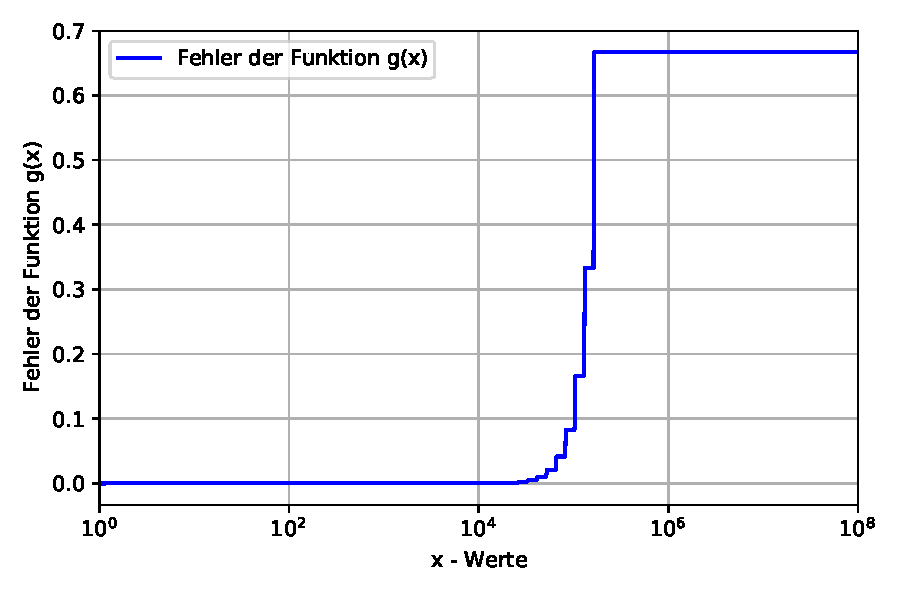
\includegraphics{build/Graph_b.pdf}
    \caption{Aufgenommene Teilchenzahl $N$ in Spannungsabhängig sowie durchgeführte Ausgleichsrechnung.}
    \label{fig:graph1}
\end{figure}


\subsection{Nachentladungen}

Die Spannung am Zählrohr wird zunächst so weit heruntergeregelt, dass am Oszilloskop kein zweiter hervorgerufener Impuls sichtbar ist.
Nachdem die Spannung auf $700 \,\unit{\volt}$ erhöht wird, sind auf dem Oszilloskop weitere Impulse sichtbar, die Nachentladungen.
Mithilfe von \autoref{fig:messung2} bestimmt sich der Abstand zwischen Primär- und Nachentladung dabei zu ungefähr $200 \,\unit{\micro\second}$.

\begin{figure}
    \centering
    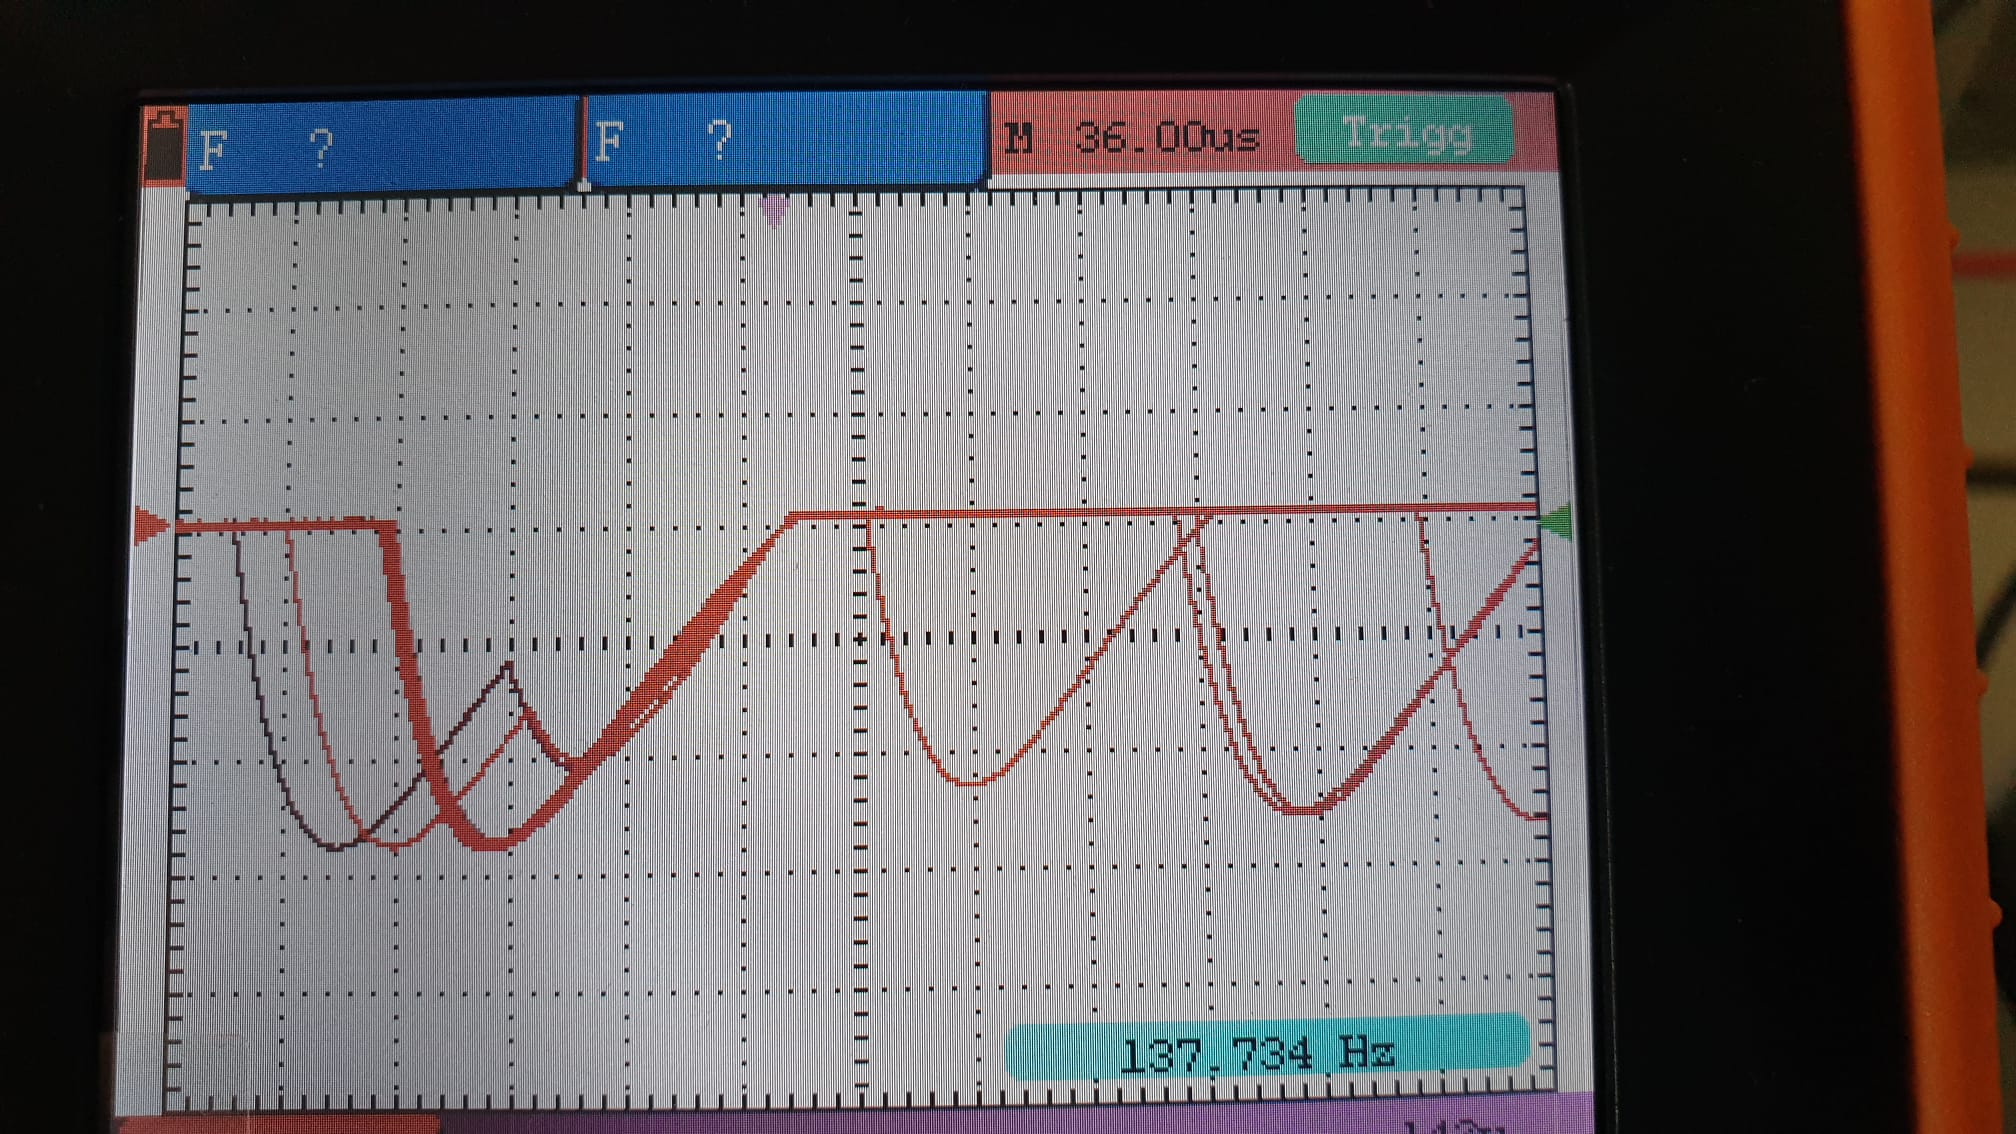
\includegraphics[scale=0.2]{figures/messung2.jpeg}
    \caption{Primär- und Nachentladungen bei $U = 700 \,\unit{\volt}$ bei $50 \,\unit{\micro\second}$ pro Kästchen.}
    \label{fig:messung2}
\end{figure}


\subsection{Bestimmung der Totzeit}

Aus \autoref{fig:messung2} lässt sich neben dem Abstand zwischen Primär- und Nachentladungen auch die Totzeit ablesen.
Die beträgt dabei ungefähr $2,5$ Kästchen, also
\begin{equation*}
    T \approx 125 \,\unit{\micro\second} \,.
\end{equation*}

Genauer kann sie jedoch über die Zwei-Quellen-Methode bestimmt werden.
In \autoref{tab:messung3} sind dabei die Teilchenzahlen der beiden Einzelquellen sowie beider Quellen gemeinsam, erneut auf einem Intervall von $120 \,\unit{\second}$ mitsamt der nach \eqref{eq:totzeit} berechneten Totzeit dargestellt.

\begin{table}[H] %% Der Wert der Totzeit stimmt hier nicht, dass war glaube ich das, was du Donnerstag gesagt hattest, oder? 
    \centering
    \caption{Teilchenzahlen der Quellen sowie Totzeit $T$.}
    \label{tab:messung3}
    \begin{tabular}{|S | S|}
      \hline
        {$N_1$ in $\dfrac{1}{\unit{\second}}$}                             &  {$184,0 \pm 1,2$}  \\
        \hline
        {$N_{1 + 2}$ in $\dfrac{1}{\unit{\second}}$}                      &  {$336,3 \pm 1,7$}    \\
        \hline
        {$N_2$ in $\dfrac{1}{\unit{\second}}$}                             &  {$157,2 \pm 1,1$}    \\
        \hline
        {$T \mathbin{/} \unit{\second}$}    &  {$(8,6 \pm 4) \cdot 10^{-05}$} \\
    \hline
    \end{tabular}
\end{table}


\subsection{Freigesetzte Ladung pro Teilchen}
\label{subsec:ladung}


\begin{table}[H]
    \centering
    \caption{Eintreffende Teilchenzahl $N$ in Abhängigkeit der Spannung $U$.}
    \label{tab:messung4}
    \begin{tabular}{S[table-format=3.0] S[table-format=1.3] S  S}
      \toprule
        {$U \mathbin{/} \unit{\volt}$} & {$I \mathbin{/} \unit{\micro\ampere}$} & {$\Delta Q \mathbin{/} 10^{-9}\unit{\coulomb}$} & {$10^{10} \, \frac{\Delta Q}{\text{e}}$} \\
      \midrule
      350  &  0.200 &  {$1,63 \pm 0,16$} &  {$1,02  \pm 0,10$}       \\
      360  &  0.150 &  {$1,24 \pm 0,17$} &  {$0,77 \pm 0,10)$}       \\
      370  &  0.175 &  {$1,42 \pm 0,16$} &  {$0,88 \pm 0,10)$}       \\
      380  &  0.200 &  {$1,61 \pm 0,16$} &  {$1,01 \pm 0,10$}       \\
      390  &  0.200 &  {$1,63 \pm 0,16$} &  {$1,02 \pm 0,10$}       \\
      400  &  0.220 &  {$1,77 \pm 0,16$} &  {$1,11 \pm 0,10$}       \\
      410  &  0.220 &  {$1,80 \pm 0,16$} &  {$1,12 \pm 0,10$}       \\
      420  &  0.250 &  {$2,03 \pm 0,16$} &  {$1,27 \pm 0,10$}       \\
      430  &  0.300 &  {$2,45 \pm 0,16$} &  {$1,53 \pm 0,10$}       \\
      440  &  0.350 &  {$2,80 \pm 0,16$} &  {$1,74 \pm 0,10$}       \\
      450  &  0.360 &  {$2,92 \pm 0,16$} &  {$1,82 \pm 0,10$}       \\
      460  &  0.380 &  {$3,12 \pm 0,17$} &  {$1,95 \pm 0,10$}       \\
      470  &  0.380 &  {$3,05 \pm 0,16$} &  {$1,91 \pm 0,10$}       \\
      480  &  0.400 &  {$3,23 \pm 0,16$} &  {$2,02 \pm 0,10$}       \\
      490  &  0.400 &  {$3,23 \pm 0,16$} &  {$2,02 \pm 0,10$}       \\
      500  &  0.410 &  {$3,30 \pm 0,16$} &  {$2,06 \pm 0,10$}       \\
      510  &  0.400 &  {$3,28 \pm 0,17$} &  {$2,05 \pm 0,10$}       \\
      520  &  0.450 &  {$3,62 \pm 0,16$} &  {$2,26 \pm 0,10$}       \\
      530  &  0.500 &  {$4,04 \pm 0,17$} &  {$2,52 \pm 0,10$}       \\
      540  &  0.500 &  {$4,05 \pm 0,17$} &  {$2,53 \pm 0,10$}       \\
      550  &  0.500 &  {$4,01 \pm 0,16$} &  {$2,51 \pm 0,10$}       \\
      560  &  0.500 &  {$3,99 \pm 0,16$} &  {$2,49 \pm 0,10$}       \\
      570  &  0.500 &  {$3,97 \pm 0,16$} &  {$2,48 \pm 0,10$}       \\
      580  &  0.580 &  {$4,69 \pm 0,17$} &  {$2,93 \pm 0,10$}       \\
      590  &  0.600 &  {$4,74 \pm 0,16$} &  {$2,96 \pm 0,10$}       \\
      600  &  0.600 &  {$4,79 \pm 0,16$} &  {$2,99 \pm 0,10$}       \\
      610  &  0.600 &  {$4,71 \pm 0,16$} &  {$2,94 \pm 0,10$}       \\
      620  &  0.600 &  {$4,76 \pm 0,16$} &  {$2,97 \pm 0,10$}       \\
      630  &  0.620 &  {$4,88 \pm 0,16$} &  {$3,04 \pm 0,10$}       \\
      640  &  0.600 &  {$4,81 \pm 0,17$} &  {$3,00 \pm 0,10$}       \\
      650  &  0.600 &  {$4,71 \pm 0,16$} &  {$2,94 \pm 0,10$}       \\
      660  &  0.600 &  {$4,67 \pm 0,16$} &  {$2,92 \pm 0,10$}       \\
      670  &  0.600 &  {$4,62 \pm 0,16$} &  {$2,89 \pm 0,10$}       \\
      680  &  0.700 &  {$5,42 \pm 0,16$} &  {$3,38 \pm 0,10$}       \\
      690  &  0.800 &  {$6,10 \pm 0,16$} &  {$3,81 \pm 0,10$}       \\
      700  &  0.750 &  {$5,74 \pm 0,16$} &  {$3,58 \pm 0,10$}       \\ 
    \bottomrule
    \end{tabular}
\end{table}

Im folgenden Graphen \autoref{fig:messung3g} ist $ \unit{\volt}$ gegen $\Delta Q \mathbin{/} \unit{\coulomb}$ aufgetragen.
\begin{figure}[H]
  \centering
  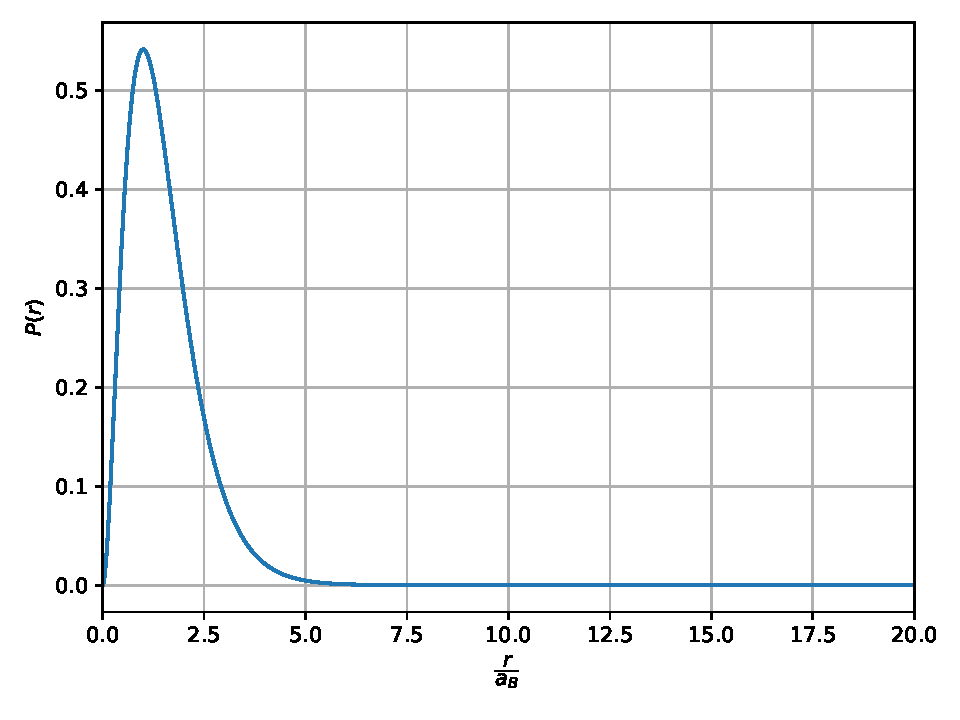
\includegraphics{build/Graph_c}
  \caption{Ladungsunterschied $\Delta Q \mathbin{/} \unit{\coulomb}$ in Spannungsabhängig sowie Ausgleichsgerade.}
  \label{fig:messung3g}
\end{figure}

Die Ausgleichsgerade 

\begin{equation*}
   y = m x + b
\end{equation*}

hat die Koeffizienten

\begin{equation*}
  a = \left( 1,24 \cdot 10^{-11} \pm 0,40 \right) \unit{\dfrac{\coulomb}{\volt}}
\end{equation*}
und

\begin{equation*}
  b = \left( -2,92 \cdot 10^{-9} \pm 183,23 \right) \unit{\volt \, .}
\end{equation*}
